\subsection{Biologie (coefficient 1.5)}

\subsubsection{Déroulement de l'épreuve}

Comme pour les deux autres épreuves de sciences, il s’agit de vérifier tes connaissances biologiques précises et d’évaluer ta capacité de synthèse, d’explication, de réflexion face à un problème et de réactivité aux questions. Tu verras souvent mentionné que le plus important est d’être motivé et vif : c’est faux, le plus important est d’avoir des connaissances solides, c’est la condition obligatoire pour que le jury envisage même de retenir ta candidature.\\

L’examinateur commence par se présenter et explique bien le déroulement de l’épreuve : il est là pour vérifier que tu possèdes les connaissances de base qui sont nécessaires (que normalement tu as si tu es là). Tu commences par \textbf{piocher deux sujets} et tu en \textbf{choisis un}. Tu as ensuite 30 minutes de préparation avec un brouillon au fond de la salle, pendant que la personne d’avant passe à l’oral : pour ceux qui sont dérangés par le bruit, pensez à prendre des boules quiès. Le prof te propose de faire des schémas sur ton brouillon pour lui montrer pendant ton exposé (donc pense à les rendre clairs directement si c’est ton intention et à apporter des stylos de couleur) ou directement au tableau pendant que tu présentes.\\

Dans un deuxième temps, tu te présentes devant le professeur qui te demande d’écrire ton plan et ta problématique au tableau pendant qu’il accueille le candidat suivant. Puis, dépendant des candidats, le prof commence par poser des questions générales pour te mettre à l’aise, comme d’où tu viens, si tu sais déjà quel domaine de recherche t'intéresse... \\

Ensuite il te demande de commencer, et tu as 15 minutes pour dérouler ton plan sur le sujet choisi, en t'appuyant sur tes schémas.\\

Finalement, c’est sûrement la partie la plus importante, le prof te pose des questions pendant 15 minutes, qui seront d’abord liées à ton sujet et qui peuvent ensuite s’en éloigner comme tu le verras dans les témoignages. Comme le prof l’explique très bien au début de l’épreuve, il pose trois types de questions : celles auxquelles il attend une réponse, celles sur lesquelles il te demande de réfléchir mais pour lesquelles il est conscient que tu n’as pas forcément la réponse à ton niveau, et celles auxquelles personne n’a encore de réponse et où il te demande donc de formuler des hypothèses. Donc ne panique pas si tu trouves certaines questions trèèès difficiles.\\

Le plus important pour cette épreuve est que ta présentation soit claire et soutenue par des exemples concrets (des notions d’expériences historiquement importantes peuvent être utiles), et n’oublie pas que contrairement à beaucoup de tes épreuves de première année de médecine, c’est un oral, donc si tu as la possibilité de t'entraîner au moins une fois (avec un prof, des amis, tes parents ou au pire avec tin chat), fais-le ++.\\

Voici une liste de sujets relativement redondants : 

\begin{itemize}
\item La mitochondrie
\item Le chromosome eucaryote
\item Communication intracellulaire
\item Communication intercellulaire 
\item Le cytosquelette
\item Le transport membranaire
\item La membrane plasmique
\item Traduction et repliement des protéines
\item Transcription et régulation de l’expression des gènes 
\item Transcription et ARN
\item Diversité du génome et variabilité génomique
\item Réplication et réparation de l’ADN
\item Edition du génome
\item Cytokines, chimiokines, hormones
\item Le noyau eucaryote
\item Le développement embryonnaire et les cellules souches
\item L’inflammation
\item Flux entre cytoplasme et noyau
\item Les antibiotiques
\end{itemize}

\subsubsection{Témoignages}

\lettrine{{\color{violet} \oldpilcrowfive}}{}
J’avais comme sujet : \textbf{la phagocytose} ou $\underbrace{\textbf{le cytosquelette : composition, structure, fonction}}_{\text{choisi}}$\\
De manière globale, je pense que c’est cool si vous avez des idées d’expériences, les expériences historiques par exemple. Et bien connaître les méthodes pour les questions.\\
Mon plan était un peu nul, mon schéma c’était une cellule où j’avais représenté les différents éléments du cytosquelette et aussi les jonctions par exemple. Je pense par contre que mon exposé était relativement complet.\\

Mon plan c’était quelque chose comme ça :\\





\begin{tikzpicture}
\draw(0,0) node{
\begin{minipage}{0.5\linewidth}
\vspace{0cm}
\begin{enumerate}[label=\textcolor{red}{\bf \Roman{*}.}]
    \item {\bf \textcolor{red}{Composition}}
    \begin{enumerate}[label=\alph*)]
        \item Actine
        \item Microtubules
        \item Filaments intermédiaires
    \end{enumerate}
    \item {\bf \textcolor{red}{Rôle dans la dynamique cellulaire}}
    \begin{enumerate}[label=\alph*)]
        \item Mouvement et forme de la cellule
        \item Déplacements au sein de la cellule
        \item Jonction cellulaire (\& communication)
    \end{enumerate}
    \item {\bf \textcolor{red}{Rôle dans la division cellulaire}}
\end{enumerate}
\end{minipage}
};

\draw[color=black,decorate,decoration={brace,raise=0.1cm}, color=green!60!black]
  (2.3,2) --++ (0,-1.5) node[right=0.2cm,pos=0.5] {\begin{minipage}{0.5\linewidth}
      \footnotesize J'ai décrit à chaque fois la forme, la polymérisation, la taille (vraiment important de connaître les ordres de grandeur), les sous-types, les caractéristiques physiques...
  \end{minipage}};

\draw[->,>=latex, color=green!60!black](3.5,-.4)--++(.5,0)node[right]{\footnotesize Actine + lamine et des exemples...};

\draw[->,>=latex, color=green!60!black](3.(3.5,-0.95)--++(.5,-.05)node[right, yshift=-.15cm]{\begin{minipage}{0.4\linewidth}
\footnotesize Les microtubules, avec le fonctionnement des moteurs moléculaires
\end{minipage}};

\path [->,>=latex, color=green!60!black] (3.2,-1.8) edge[bend right] node [left] {} (3.8,-2)node[right=.6cm, yshift=-0.5cm]{
\begin{minipage}{0.4\linewidth}
    \footnotesize Les différentes jonctions, celles qui sont reliées à l’actine ou aux filaments intermédiaires…
\end{minipage}
};

\path[->,>=latex, color=green!60!black] (1.1,-2.7) edge[bend right]node [left]{} (3,-3.2) node[right=1.9cm, yshift=-.7cm]{
\begin{minipage}{0.5\linewidth}
    \footnotesize Rôles de l’actine, les microtubules avec les différents types, les filaments intermédiaires avec les
lamines
\end{minipage}
};
\end{tikzpicture}

\bigskip

Quant aux questions posées après ma présentation, elles ont direct été assez compliquées, il m’a demandé comment ça se fait que la kinésine et la dynéine vont dans la bonne direction, comment les molécules d’actine globulaire allaient de l’autre côté de la cellule lors d’un changement de direction. J’ai fait des suppositions, j’ai réfléchi à partir de ce que je savais\dots \\
Juste avant les questions sur la bio, il m’a demandé d’où je venais, ce qui m’intéressait dans la recherche (c’est de ne plus avoir de patients ? \textbf{NON}), si j’étais en stage… C’était intéressant de discuter
avec lui et il était attentif à mes motivations aussi pour la médecine (comme je lui ai dit que mon domaine d’intérêt en recherche c’était pas mal la neuro, il m’a demandé pourquoi et j’ai parlé de la
médecine…).\\

\lettrine{{\color{yellow!80!black} \oldpilcrowfive}}{}
J’ai choisi le sujet « le transport transmembranaire » (je ne me rappelle plus mon deuxième sujet).\\
Au départ j’étais très contente de mon sujet parce que j’avais préparé une fiche-plan à ce sujet et je m’en rappelais assez bien. Mais au fur et à mesure de ma préparation je me suis rendue compte que le plan que j’avais préparé étais un peu bateau et j’étais tiraillé entre le fait de recommencer tout à zéro et le temps qui passait. Au final j’ai fait à peu près le même plan que celui que j’avais
préparé en avance mais je n’en suis pas tout à fait satisfaite…\\

\textbf{\uline{Introduction}}\\
La structure membranaire : la nécessité de mécanismes pour faire communiquer deux environnements qui doivent rester séparés\\

\begin{enumerate}[label=\color{red}{\bf \Roman*.}]
    \item {\bf \color{red} Le transport passif}
    \begin{itemize}
        \item Les ordres de grandeurs de la diffusion / dépendance de l’hydrophobicité
        \item Gradient électrochimique !!!
        \item Diffusion facilitée par les pores (saturable)
    \end{itemize}
    \item {\bf \color{red} Le transport actif}
    \begin{itemize}
        \item La pompe Na/K ATPase : gradient électrochimique
        \item Le transport actif secondaire : symport et antiport
    \end{itemize}
    \item {\bf \color{red} Endo/trans/exocytoses}
    \begin{itemize}
        \item Constitutive ou provoquée
        \item Exemple des synapses
    \end{itemize}
\end{enumerate}

\vspace{.5cm}

Après j’ai eu pas mal de questions pour lesquelles je ne connaissais pas du tout la réponse.
\begin{itemize}
    \item Comment les virus ou bactéries réussissent à pénétrer dans la cellule ?
    \item Ordre de grandeur des virus et bactéries en comparaison avec celle des pores
    \item Comment on arrive à faire entrer des médicaments ?
    \item En tant que chercheuse, quelle mécanismes privilégierez-vous ?
    \item Comment ça marche à l’intérieure de la cellule au niveau des différents compartiments ?
\end{itemize}

À la fin on a parlé un peu de mon stage. Il a essayé de faire un lien entre mon stage et le sujet.\\
C’était compliqué pour lui de trouver, mais comme ça il m’a posé des questions un peu bateau.\\

Quelque chose de vraiment important je pense, ce sont les ordres de grandeur. Je vous mets ma fiche récap que j’avais fait si ça peut
vous aider.

\begin{center}
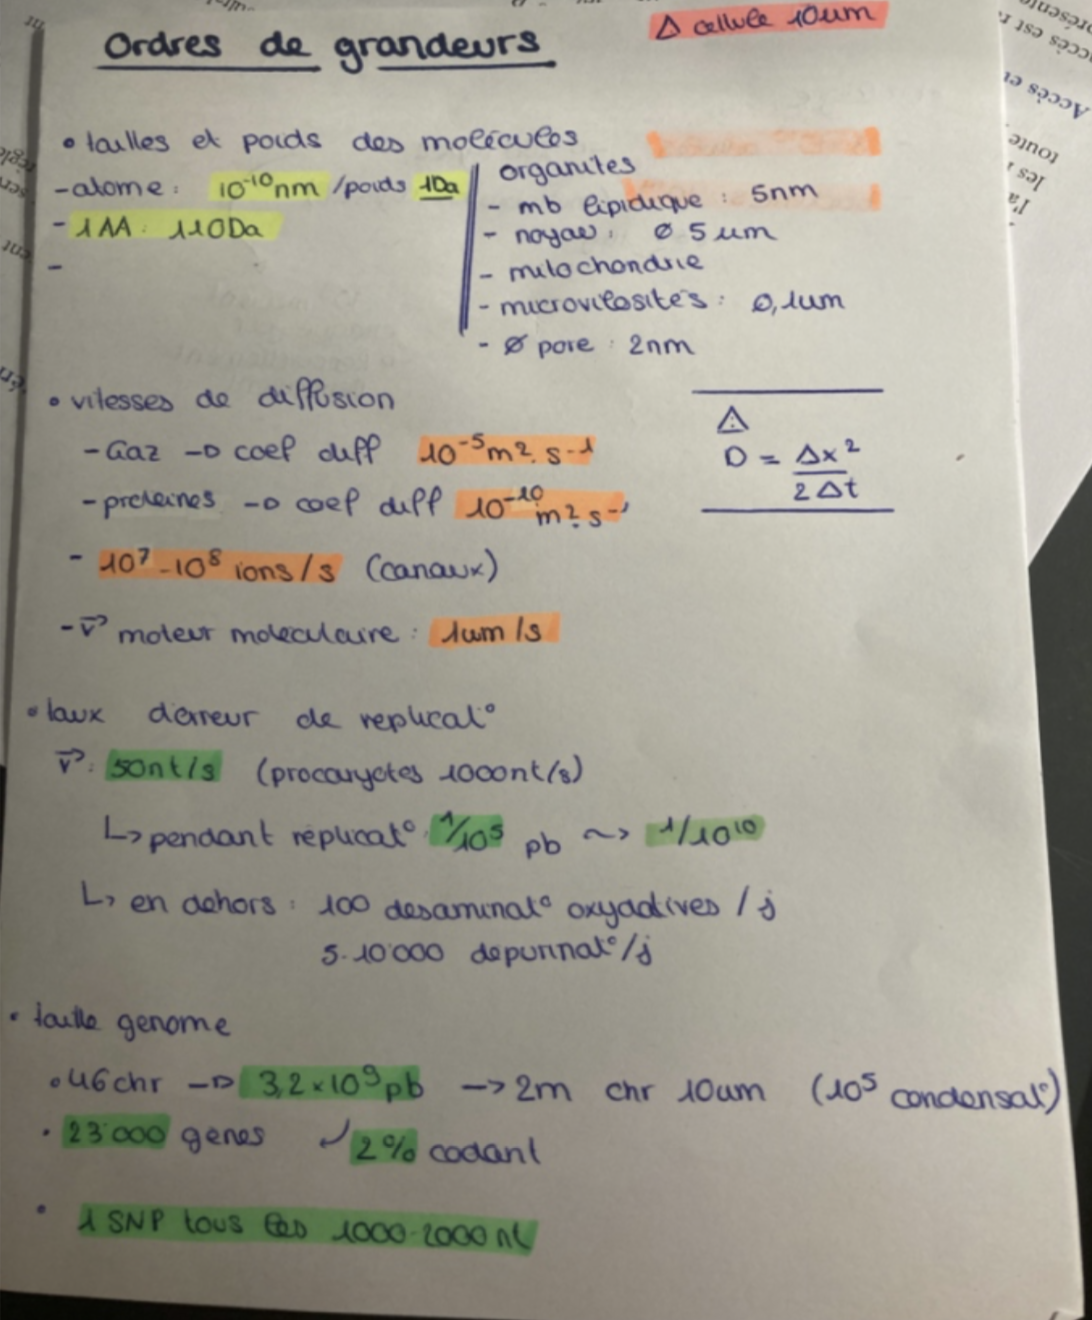
\includegraphics[width=7cm]{fiche.png}
\end{center}

Courage à vous, ce n’est pas une
période facile mais vous êtes des
guerriers !!!!!!\\


\lettrine{{\color{violet} \oldpilcrowfive}}{}
Dernier entretien de la série. L'examinateur est vraiment incroyable, et on a plus l'impression de discuter pendant 40 min que de passer un vrai oral de bio basé sur nos conséquences. \\
J'ai pioché 3 sujets complétement étranges et qui ne me mettaient pas du tout en confiance (Orage cytokinique et cancer ? SIDA ?). Il m'a très gentiment laissé repiocher jusqu'à ce que je tombe sur un sujet bien bateau : "Gènes et évolution des génomes". Je lui ai sorti un plan très peu structuré, avec des schémas de chromosomes, où je racontais globablement ce qui me passait par la tête :

\begin{enumerate}
\item Microinstabilité satellite
\item Remaniements chromosomiques
\item Évolution et pression de sélection (où j'expliquais la méiose et la fécondation ?)
\end{enumerate}

\vspace{.25cm}

Après avoir écrit ce ravissant plan au tableau, j'ai présenté mon sujet pendant une dizaine de minutes. Lui et moi voyions bien que ce n'était absolument pas préparé, mais il m'a laissé finir. Nous avons donc très vite enchaîné sur des questions de réflexion, qui ressemblaient plus à une discussion qu'autre chose, je n'ai pas vu le temps passer et c'était vraiment très agréable. Après m'avoir demandé rapidement qui j'étais et ce qui m'intéressait dans la vie (questions que je n'ai pas eues dans mon entretien de motivation), il a axé ses questions sur de la génétique des populations et de l'évolution. On avait l'impression qu'il réfléchissait en même temps que moi, que lui non plus n'avait pas la réponse et que tout ce qui importait était la réflexion. \\

Il m'a demandé quelques ordres de grandeur sur le génome, sur les temps caractéristiques en évolution... Je n'y connais absolument rien en génétique, mais je crois que c'est ce qu'il cherchait. Il m'a demandé aussi ce qui se passerait si on scindait une population en 2 (dérive génétique ?) et ce sur quelle échelle de temps. Il voulait aussi savoir ce que je pensais de la maladie, notamment en virologie, et s'il était envisageable qu'on soit un jour vacciné contre tout : les maladies disparaitraient-elles ? Certaines questions étaient parfois plus axées philo que bio, c'était assez étonnant : l'homme doit-il maîtriser la nature ?..\\

Je suis sorti assez content de cet oral, je n'avais pas beaucoup de connaissances mais nous avons tout de même pu avoir une vraie discussion, nous poser des questions sérieuses et pertinentes. L'interrogatoire était vraiment super bien mené. Niveau préparation, je pense qu'il est toujours pertinent d'avoir revu tout le programme bio de BCPST/P1, mais avec cet examinateur, la culture générale et la réflexion comptent aussi énormément, pouvant expliquer les sujets un peu hors-programme au premier abord. \\

\lettrine{{\color{yellow!80!black} \oldpilcrowfive}}{}
J’ai eu un sujet sur \textbf{la variabilité de la synthèse protéique et la régulation de la transcription} (pas exactement ça mais dans le style, c’était assez classique). L’oral de bio est celui que j’ai le plus aimé, l’idée c’est vraiment de vous éclater en discutant de sujets qui vous passionnent autour de la bio. La partie khôlle de prépa n’est là que pour construire l’entretien dessus, car l’examinateur assume qu’en médecine on a déjà plein de connaissances acquises par cœur, l’objectif étant à présent de voir ce qu’on sait en faire. Le meilleur conseil que je peux vous donner en bio, en dehors de faire une présentation potable et de réfléchir à voix haute aux questions qu’on vous aura données auxquelles vous n’aurez certainement pas la réponse, c’est de vous-même orienter l’entretien vers votre domaine de prédilection et de PROFITER. L’examinateur est lui-même ici parce qu’il adore discuter avec des étudiants passionnés, et de montrer cet intérêt et de mener la conversation vers ce qui vous plaît vraiment vous évitera les questions bidon du type : combien il y a-t-il de mitochondries dans un fibroblaste ? Perso j’ai pu avoir une discussion très intéressante sur les CAR-T et le cancer. Note : 16.\\

\newpage
\lettrine{{\color{violet} \oldpilcrowfive}}{}
\textbf{Sujets tirés :} \uline{La communication intracellulaire} ou \uline{les antibiotiques}\\
\textbf{Sujet retenu : communication intracellulaire}\\

Voici mon plan :

\begin{enumerate}[label=\textcolor{red}{\bf \Roman*.}]
    \item {\bf\color{red} La communication intracellulaire permet le transport et bonne localisation des constituants cellulaires}
    \begin{enumerate}[label=\alph*)]
        \item Communication impliquée dans le bon adressage des protéines aux compartiments cellulaires
        \item Le transport intracellulaire permet la communication entre les composants cellulaires
    \end{enumerate}
    \item {\bf\color{red}L’émission de signaux en réponse aux dommages à l’ADN, un élément central de la communication intracellulaire}
    \begin{enumerate}[label=\alph*)]
        \item Les différents types de dommages à l’ADN
        \item La cascade de signalisation des dommages de l’ADN
    \end{enumerate}
    \item {\bf\color{red}Les conséquences cellulaires de la voie de signalisation des dommage à l’ADN}
    \begin{enumerate}[label=\alph*)]
        \item Arret du cycle cellulaire
        \item Déclenchement de l’apoptose
    \end{enumerate}
\end{enumerate}

Quant à la partie questions, le prof a commencé par des questions assez simples faisant appel à des connaissances notamment sur les récepteurs à tyrosine kinase et leurs modes de transduction, aux autres types de récepteurs et a ensuite élargi le sujet en posant des questions sur d’éventuelles implications physiopathologiques/pharmaceutiques et d’imaginer des approches pour l’étude ou le développement de médicaments concernant des altérations de différentes voies de signalisation.\\
L’examinateur est très aimable et met à l’aise mais il sait aussi rester neutre donc il est difficile de savoir si ce qu’on dit est pertinent ou si on est complètement à côté de la plaque.\\



\lettrine{{\color{yellow!80!black} \oldpilcrowfive}}{}
\uline{Sujets :} Auto-immunité / immunité adaptative / \textbf{Inflammation (retenu)}\\
Alors, oui j’ai pioché tous les sujets d’immuno du paquet... alors que j’avais révisé... tous sauf l’immuno. Il m’a donc laissé pioché 3 sujets (quand il a vu ma tête), mais j’ai réussi à piocher le troisième sujet d’immuno. Si si, Je pleurais un peu intérieurement.\\
Il m’a rassurée en m’expliquant que la présentation c’est juste pour introduire la discussion, le sujet et que c’était vraiment la discussion qui vient après le plus important. Retenez bien ça !\\
J’ai jeté au brouillon tous mes souvenirs de l’inflammation depuis la terminale à la P2 et ensuite j’ai organisé un plan autour de ça. J’étais assez vague parfois (à mon avis) et dès que il y avait quelque chose que je connaissais bien, je fais une sorte de « zoom » dessus, pour étaler mes connaissances etc... Donc je crois que j’ai tenu 15min.\\
Le prof commence par se présenter et vous demande de vous présenter, on a même parlé de ce que je faisais pendant mon stage. Ça met vraiment à l’aise. Il me répète que la présentation n’est pas le plus important etc...\\

\uline{\textbf{Petite intro :}} \\
$\longrightarrow$ Définition de l’inflammation : réaction stéréotypée (rougeur / chaleur / douleur / oedème) mise en place par l’organisme face à une agression extérieur (infection) ou intérieure (cancer)\\

\uline{\textbf{Problématique :}} Quels sont les mécanismes de la réaction inflammatoire ?\\
C’est un peu bateau, j’avais pas trop d’inspiration et je m’étais plutôt concentrée sur le contenu, en me disant que je verrai après pour la problématique. Ne perdez pas du temps dessus, si ça vous n’avez rien en tête. Préparez d’abord votre plan et voyez ce qui ensuite peut bien marcher.\\

\begin{enumerate}[label=\textcolor{red}{\bf\Roman*.}]
    \item {\bf\color{red}Les acteurs de la réaction inflammatoire}
    \begin{enumerate}[label=\alph*)]
        \item Signaux de danger : PAMP / DAMP (Gram + gram - etc) reconnus par PRR / TLR / NLR
        \item Acteurs cellulaires : PNN / PNE / PNB / CPA / Macrophages (J’ai rapidement passé en revue le rôle de chacun)
        \item Inflammasome : NF$\kappa$B / IL1 / caspases\\
        {\color{green!60!black}$\longrightarrow$ \textit{(j’ai détaillé le système caspasaine / calpastatine parce que je l’avais vu dans mes révisions, donc autant que ça serve à quelque chose)}}
        \item Acteur soluble, le complément : 3 voies (classique / alterne / lectines) C6/7/8/8 = Complexe de lyse membranaire et C3a et C5a très inflammatoires.\\
        {\color{green!60!black}\textit{$\longrightarrow$ Je n’ai pas présenté toute le cascade, et ce n’est certainement pas ce qu’ils attendent de nous ! Ne vous embourbez pas dans des détails superflus. J’avais un schéma franchement pas beau sur le brouillon d’un épithélium avec une épine, 3 cellules qui se baladent, un vaisseau et une bactérie avec des triangles sur la membrane (vous voyez le genre). Essayez d’avoir quelque chose d’assez claire, car il nous demandait de lui montrer nos schémas sur le brouillon et pas de les refaire au tableau.}}
    \end{enumerate}
    \item {\bf\color{red}Recrutement des cellules immunitaires sur le lieu de l’inflammation}\\
    {\color{green!60!black}\textit{$\longrightarrow$ J’ai détaillé les cytokines / chémokines, et j’avais fait le schéma sur le brouillon roulement / reptation et touticouanti des leucocytes.}}
    \item {\bf\color{red}Rôle de l’inflammation dans les pathologies}\\
    {\color{green!60!black}\textit{$\longrightarrow$ C’était plus une ouverture qu’une vraie 3ème partie. J’ai pris pour exemple différentes pathologies vues en cours, qui avaient un lien avec l’inflammation.
    \begin{itemize}
    \item Inflammation et cancer $\Rightarrow$ L'’inflammation est-elle favorable ou défavorable ? 
    \item MICI : Maladie Inflammatoire Chronique de l’Intestin $\Rightarrow$  Interaction entre microbiote et système immunitaire 
    \item La goutte : Rôle de l’inflammasome, et traitement : Inhibiteur d’IL1-RA
    \end{itemize}}}
\end{enumerate}

Il m’a dit : « Bon bah c’était plutôt pas mal pour quelqu’un qui n’avait pas préparé ! » et on est passé aux questions :\\

\begin{enumerate}[label=\blacksquare]
    \item \uline{\textbf{De cours :}} 
    \begin{itemize}
        \item "Pourquoi les cytokines ont-elles une durée de vie aussi faible ?" \\
        $\longrightarrow$ soit $\approx$ 30min, je l’avais dit dans l’exposé, rappelez-vous, ils kiffent les ordres de grandeur, donc plus vous en dites dans l’exposé, moins ils vous en poseront — je pense — dans la période des questions
        \item "Une fois dans le vaisseau sanguin, les chémokines, avec le flux sanguin, risquent d’être emportées, donc quand elles vont se fixer sur les leucocytes, ne risquent-elles pas d’être « décalées » par rapport au site de l’inflammation ?"\\
        $\longrightarrow$ J’ai expliqué que d’une part le flux était presque nul près de la paroi au niveau de l’endothélium et d’autre part, le roulement des leucocytes se fait à l’état basal, cad sans inflammation, en état de surveillance, lorsque les chémokines passent l’endothélium, elles rentrent rapidement en contact avec un leucocyte, donc avant de se retrouver au milieu du vaisseau où le flux est important.\\
        J’ai dit que comme c’était des molécules solubles, elles étaient instables en milieu aqueux. (Je sais pas si c’est la réponse)
    \end{itemize}
    \item \uline{\textbf{Le reste :}}  Je vais essayer de retranscrire le reste sous forme de questions-réponses, mais c’était vraiment plus un échange :
    \begin{itemize}
        \item "Vous avez dit que vous aimiez la rhumatologie, pourquoi est-il important de savoir reconnaitre les signes de la réaction inflammatoire dans cette discipline ?"\\
        $\longrightarrow$ J’ai dit que cela permettait d’identifier différentes pathologies mécaniques VS inflammatoires, donc différentes origines etc... Et que l’inflammation pouvait aussi aggraver une pathologie comme l'arthrose.\\
        \item "Vous avez parlé d’inhibiteur d’IL1 dans le traitement de la goutte, ce traitement permet-il de guérir la pathologie ou l’inflammation ?\\
        $\longrightarrow$ Cela permet juste de diminuer les effets de l’inflammation, notamment la douleur, mais pas l’origine de la pathologie étant l’excès d’acide urique.
        \item "Si ça ne permet pas de guérir la pathologie, alors pourquoi ce traitement est-il utilisé ?" \\
        $\longrightarrow$ J’ai dit que la goutte pouvait très bien être occasionnelle (quelqu'un qui a mangé trop de viande) donc traiter les symptômes inflammatoires est une bonne solution dans ce cas-là mais qui ne s’appliquerait pas à un patient qui fait des crises de gouttes à répétition.\\
        J’ai souligné l’importance d’identifier la source d’une pathologie et de traiter cette dernière et pas seulement l’inflammation.
        \item On en est venu à relever la controverse des anti-inflammatoires, qui venaient masquer une pathologie en éteignant les symptômes inflammatoires, alors que l’inflammation est une réaction « physiologique » de l’organisme mise en place pour nous alerter d’un problème. J’ai cité l’exemple de l’entorse : si on prend des AINS, on ne la sentira plus, mais les ligaments continuent de se détruire, et ça deviendra irréversible etc...\\
        Cependant, l’inflammation peut devenir pathologique, d’où l’intérêt des AINS, qui est le seul traitement antalgique ciblant l’inflammation par l’inhibition des prostaglandines. \\
        Au final, ça m’ait venue après mais j’aurais pu dire : « Les antibiotiques c’est pas automatique, et les anti-inflammatoires, c’est pas obligatoire ». C’est plus ou moins ce que j’ai dit pendant l’oral, mais en moins stylé.
        \item Il a abordé la polyarthrite rhumatoïde (PR) comme exemple. Donc on a un peu parlé de maladie auto-immunes, et de mécanismes. J’ai dit que il y avait des mécanismes directs comme avec la PR mais aussi parfois indirects comme avec le lupus.
        \item Comme j’ai dit que je voulais faire de la médecine aérospatiale, il m’a demandé le rôle de l’inflammation en apesanteur. Il m’a un peu guidée pour me faire dire qu’en apesanteur, comme on n’a plus de contraintes, qui permettent justement de modeler le cartilage, celui-ci risque de « grandir » et donc être source d’inflammation au retour sur terre par exemple.
        \item "Vous avez parlé des MICI, que savez-vous ? D’où connaissez-vous cette pathologie ?"\\
        $\longrightarrow$ J’ai expliqué que ces pathologies avaient des causes environnementales, auto-immunes, et de déséquilibre avec le microbiote. J’ai dit que j’avais découvert cette pathologie sur internet parce que ça m’intéressait et lors de mon stage en soins infirmiers au service de chirurgie colorectale.
        \item Du coup on a fait une grosse parenthèse stage de médecine et m’a demandé quelles pathologies il y avait dans le service : Maladie de Chron, RCH et cancer colorectaux.
        \item "Stades de polype ?"\\
        $\longrightarrow$ J’ai dit que pour le coup c’était plus le stade carcinose péritonéale (donc très avancé) et j’ai fini par décrire l’opération à laquelle j’avais assisté une CHIP (Chimiothérapie Hyperthermique Intra-Péritonéale). Rien à voir avec l’oral, très clairement, mais il était super intéressé.
        \item Puis on est revenu au sujet : "Vous parlez d’interaction avec le microbiote, pourquoi ?"\\
        $\longrightarrow$ J’ai parlé des greffes de matières fécales qui prouvaient qu’il y avait bien une interaction entre le système immunitaire et le microbiote, et une notion d’équilibre / déséquilibre. Et on a parlé de ça pendant plusieurs minutes. J’ai abordé les complications puisqu’en effet si cellule de soi (CMH) alors peut-être microbiote du soi, donc rejet de greffe etc... Il m’a dit que, oui, ça existait et qu’il pouvait y avoir des rejets.
        \item Il m’a demandé si j’avais vu ça en cours. J’ai dit que je ne m’en rappelait pas, sûrement un reportage mais si ça se trouve, c’était peut-être un Sciences et Vie Junior. Mais pas en cours étant donné que l'UE de digestif est en D1 dans ma fac. Il était un peu déçu aha, parce que si c’était dans nos cours, ça aurait voulu dire que la recherche dans ce domaine là avait beaucoup avancé. En tous cas, d’après lui beaucoup de recherche sont faite dans le domaine.
    \end{itemize}
\end{enumerate}


« Franchement, pour quelqu’un qui n’avait pas préparé l’immunologie, c’est tout à votre mérite ! » (Bon j’ai su que ça avait peut-être mal commencé mais très bien terminé, donc faut surtout pas vous décourager et aller au bout, de belles surprises vous y attendent peut-être !).\\

Je lui répète que j’étais un peu frustrée parce qu’il y avait d’autres sujets où je possédais des connaissances très précises alors que là j’étais parfois un peu vague comme il l’avait sûrement constaté. J’ajoute en rigolant que si j’avais vraiment révisé l’immunologie comme le reste, je lui aurait dessiner toute la cascade enzymatique du complément. Ça l’a fait rire aussi.\\
Il m’accompagne dehors et dernière question sur mon stage de recherche (dans le couloir mdr), il voulait savoir si il y avait des femmes dans notre étude parce que leur adaptation était différente etc... Bref, ayez confiance en vous, même si vous avez l’impression de ne pas avoir révisé quelque chose, vous savez plein de choses, il n’y a plus qu’à leur montrer !\\


\lettrine{{\color{violet} \oldpilcrowfive}}{}
L’examinateur commence par nous expliquer le déroulé de l’épreuve et sait vraiment nous mettre à l’aise, ce qui fait que nous avions plus ou moins tous un bon ressenti en sortant. Je m’étais préparée à cette épreuve en rédigeant un plan de chacun des sujets qui tombaient le plus fréquemment. Je me suis basée sur le livre de BCPST et mes cours de PASS.\\


Sujets : \textbf{La phagocytose} ou $\underbrace{\textbf{La relation structure-fonction des protéines}}_{\text{choisi}}$

J’avais préparé le second sujet, que j’ai donc choisi sans trop hésiter.\\

\uline{\textbf{Problématique :}} Comment les protéines adoptent-elles des conformations uniques et exercent-elles des fonctions multiples nécessaires à la survie d’un organisme ?\\

\begin{tikzpicture}
\draw (0,0) node{
\begin{minipage}{0.7\linewidth}
\vspace{0cm}
\begin{enumerate}[label= \textcolor{red}{\bf \Roman*.}]
    \item \textcolor{red}{\bf De la structure primaire à la structure quaternaire des protéines}
    \begin{enumerate}[label=\alph*)]
        \item Structure $\text{\romanbar{I}}^{\text{aire}}$
        \item Structure $\text{\romanbar{II}}^{\text{aire}}$
        \item Structure $\text{\romanbar{III}}^{\text{aire}}$
        \item Structure $\text{\romanbar{IV}}^{\text{aire}}$
    \end{enumerate}
    
    \item \textcolor{red}{\bf Le repliement des protéines leur permet d’acquérir une fonction spécifique}
    \begin{enumerate}[label=\alph*)]
        \item Le repliement de la protéine est encodé dans sa structure primaire
        \item Les modèles de repliement des protéines
        \item Les protéines d’aide au repliement (chaperonnes) 
        \item Dégradation par le protéasome en cas de mauvais repliement
    \end{enumerate}
    
    \item \textcolor{red}{\bf Les protéines exercent des fonctions multiples et variées au sein de l’organisme}
    \begin{enumerate}[label=\alph*)]
        \item Les protéines fibreuses structurent la cellule
        \item Les protéines globulaires jouent un rôle important dans le métabolisme
    \end{enumerate}
\end{enumerate}
\end{minipage}
};

% partie I
%% item A
\draw[->,>=latex, color=green!60!black, shift={(-1,3.6)}] (0,0) to[out=30, in=180, looseness=1] (2,.35) node[right, fill=green!5!white]{
\scriptsize
Acide aminé (structure, pttés, fonctions) + liaison peptidique
};
%% item B
\draw[->,>=latex, color=green!60!black, shift={(-0.95,3.1)}] (0,0) to[out=30, in=180, looseness=1] (2,.45) node[right, align=left, yshift=-.15cm, fill=red!5!white]{
\scriptsize 
Hélice $\alpha$, feuillet $\beta$, coudes, boucles \\[-.1cm]\scriptsize+ Association de structures secondaires en domaines
};
%%item C
\draw[->,>=latex, color=green!60!black, shift={(-0.85,2.4)}] (0,0) to[out=15, in=180, looseness=1] (2,.4) node[right, align=left, yshift=-.15cm, fill=blue!5!white]{
\scriptsize 
Maintien de la structure tertiaire par des liaisons covalentes, \\[-.1cm] \scriptsize hydrogène, ioniques (importantes pour la fonction des protéines)
};
%%item D
\draw[->,>=latex, color=green!60!black, shift={(-0.85,1.9)}] (0,0) to[out=-15, in=180, looseness=1] (2,.1) node[right, align=left, yshift=-.15cm, fill=orange!5!white]{
\scriptsize 
Association de chaînes peptidiques\\[-.1cm]\scriptsize + Assure des fonctions biologique 
};

% Partie II
%% item A
\draw[->,>=latex, color=green!60!black, shift={(4,0.5)}] (0,0) to[out=40, in=150, looseness=1] (1.8,.2) node[right, fill=green!5!white, yshift=-.5cm]{
\begin{minipage}{0.3\linewidth}
\scriptsize
Ex : hémoglobine avec importance de la séquence d’AA montrée par la seule mutation en cause dans la drépanocytose.\\
Résidus qui peuvent acquérir des modifications post-traductionnelles qui déterminent la structure de la protéine
\end{minipage}
};
%%item B
\draw[->,>=latex, color=green!60!black, shift={(2.9,-.6)}] (0,0) to[out=10, in=190, looseness=1] (3,-.6) node[right, align=left, yshift=-.15cm, fill=orange!5!white]{
\begin{minipage}{0.25\linewidth}
\scriptsize 
Séquentiel et hiérarchique, effondrement hydrophobe, entropie 
\end{minipage}
};

%Partie III
%% item A
\draw[->,>=latex, color=green!60!black, shift={(3.4,-3.6)}] (0,0) to[out=10, in=170, looseness=1] (2.5,.2) node[right, fill=blue!5!white]{
\begin{minipage}{0.3\linewidth}
\scriptsize Collagène, kératine, protéines musculaires
\end{minipage}
};
%% item B
\draw[->,>=latex, color=green!60!black, shift={(3.4,-4.4)}] (0,0) to[out=-60, in=-160, looseness=1] (2,-.5) node[right, fill=yellow!5!white]{
\begin{minipage}{0.3\linewidth}
\scriptsize
Albumine, globuline\\
Défense de l’organisme : anticorps
\end{minipage}
};
\end{tikzpicture}

\bigskip


Vinrent ensuite les questions, divisées en trois groupes :
\begin{itemize}
    \item Celles auxquelles une réponse est attendue
    \item Celles auxquelles une réponse n’est pas forcément attendue, mais plutôt un cheminement ou une/des  hypothèses
    \item Celles auxquelles personne n’a de réponse pour l’instant (conseil pour pouvoir espérer répondre correctement à une des questions \href{https://www.youtube.com/watch?v=4xmCe_PQybE}{<ici>})
\end{itemize}

\vspace{.5cm}


Voici une partie des questions que l’examinateur m’a posées :
\begin{itemize}
    \item Comment déterminer la structure d’une protéine ?
    \item Pouvez-vous citer quelques modifications post-traductionnelles ?
    \item Comment expliquer la diversification du rôle des protéines depuis la cellule procaryote à la cellule eucaryote ? 
    \item Quelle conception avez vous d’une protéine ? (\href{https://drive.google.com/file/d/1yT1XqiO7yJkoMji1EzFvYaB0gDA03Eax/view?usp=sharing}{Je vous laisse philosopher à votre guise})
\end{itemize}



\newpage